\documentclass[twocolumn]{article}
\usepackage[top=1.1in, left=0.85in, right=0.85in]{geometry}

\usepackage{amsmath}
\usepackage{amssymb}
\usepackage{graphicx}
\usepackage{fancyvrb}
\usepackage{url}
\usepackage{textcomp}
% \usepackage{inlinebib}

\pagestyle{empty}

\newcommand\comment[1]{}

\newcommand\st{$^{\mathrm{st}}$}
\newcommand\nd{$^{\mathrm{nd}}$}
\newcommand\rd{$^{\mathrm{rd}}$}
\renewcommand\th{$^{\mathrm{th}}$}
\newcommand\tm{$^{\mbox{\tiny \textsc{tm}}}$}

% nice fractions
\newcommand\sfrac[2]{{}\,$^{#1}$\!/{}\!$_{#2}$}

\newcommand\citef[1]{\addtocounter{footnote}{1}\footnotetext{\cite{#1}}\ensuremath{^{\mbox{\footnotesize [\thefootnote]}}}}

% XXX TODO: before submit, search ``red eye'' and ``reduction'' vs removal
% we -> I

\begin{document} 

\title{Red i removal with artificial retinal networks}
\author{Dr.~Tom~Murphy~VII~Ph.D.\thanks{
Copyright \copyright\ 2015 the Regents of the Wikiplia
Foundation. Appears in SIGBOVIK 2015 with the increasingly askance visage of the
Association for Computational Heresy; {\em IEEEEEE!} press,
Verlag-Verlag volume no.~0x40-2A.
0.00 Australian Neo-Dollars}
}

\renewcommand\>{$>$}
\newcommand\<{$<$}

\date{1 April 2015}

\maketitle

\begin{abstract}
We present a GPU-accelerated means for red i removal in photographs.
\end{abstract}

\vspace{1em}
{\noindent \small {\bf Keywords}:
  computational photography, image processing, generalized photoshop, artificial retinal networks, types
}

\section{Introduction}

When light---such as the bright flashbulb of a camera---strikes the
human eye, it illuminates the retina. Some of that light bounces back
out of the eye, but most of it stimulates neurons in the retina to
produce electrical signals. These signals stimulate other neurons to
which they are connected, and so on, until the brain (which is
technically part of the eye) perceives an image, as a two-dimensional
array of neurons with different activation levels. Humans often use
these images to sense the world, for example, in reading research papers.

This research paper concerns a particular feature of this process,
which is that humans are able to view an image and ignore certain
details of it. For example, Figure~\ref{fig:cbs} contains a printout
of an image file of a photograph of a television displaying a recorded
video of an actor. The video contains a superimposed eye in the
corner, the logo of the network CBS. Most viewers are not tormented by
this everpresent eye staring at them! In fact, most viewers are able
to completely ignore the eye, and view the scene as though it didn't
contain the stimulus, even if details such as the actor's sweatshirt's
collar pass beneath the stimulus and are occluded by it.

\begin{figure}[t]
\begin{center}
\includegraphics[width=0.85 \linewidth]{cbs}
\end{center}
\caption{Q.~Who watches the TV~watchers?
A.~CBS's all-seeing eye.} \label{fig:cbs}
\end{figure}

Some stimulus is more everpresent than others. The Clay Mathematics
Institute lists among its unsolved {\em Millennium Prize} problems the
``red i removal problem.'' This concerns the removal of stimulus (a
red letter ``i'') from images (Figure~\ref{fig:redi}). The problem
is particularly difficult because the information occluded by the
i is completely gone, and because the authors of papers about the
problem are persistently agitated because it seems like the letter
should be capitalized.

In this paper I show how red i removal can be solved in certain
specialized cases, using an artificial retinal network patterned after
the brain contained within the human eye. Training this artificial
retinal network is feasible on a single powerful desktop machine. Both
training and execution of the model (a mere 400 megabytes) are GPU
accelerated. The model presented in this paper was trained in about 3
days, and executing it in parallel on a suite of images takes about
100 milliseconds per image.\!\footnote{Source code is available on
the World Wide Web at:
{\tt http://sourceforge.net/p/tom7misc/svn/HEAD/tree/trunk/redi}}

\begin{figure}[tb]
\begin{center}
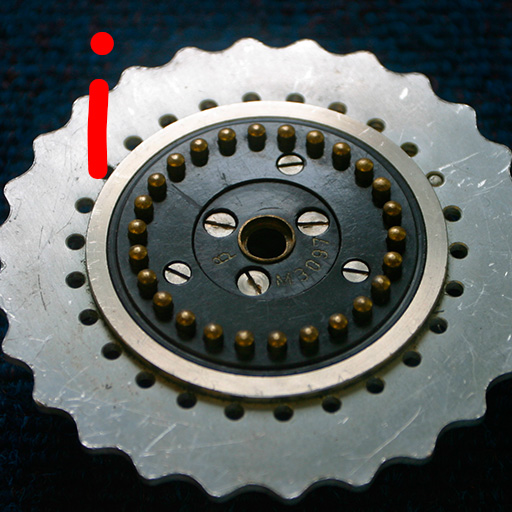
\includegraphics[width=0.65 \linewidth]{rotor}
\end{center}
\caption{An image of an Enigma machine rotor with a red i
 superimposed. Solving this instance of the red i removal problem
 would mean producing an image without the red i. One way to do this
 would be to steal a floppy disk containing an original, unimposed
 image of the rotor, from someone in possession of it, for example
 the paper's author.} \label{fig:redi}
\end{figure}

\section{Artificial retinal networks}

As I expertly foreshadowed in the previous section, an artificial
retinal network works just like the brain inside a human eye. The
retina is itself a rectangular 2D array of neurons, which turn photons
into IEEE-754 floating point values between 0.0f and 1.0f. Behind this
is another 2D array of exactly the same size, except the pixels are in
a weird jumbled order, and then another layer. This series of layers
is known as the optic nerve. Finally, the brain perceives the image as
an array of pixels, again of the same size (Figure~\ref{fig:retinal}).

It is easy to reconceptualize this process as an array of pixels
undergoing several transformations. Obviously the story is more
complicated: Humans see in color, so each pixel is actually three
different nodes, one for red, green and blue. In fact, since some
scientists hypothesize of certain ``superseers''---that is, people who
can perceive more than just the three wavelengths of light---we
actually allow an arbitrary number of nodes per pixel. In this work,
we used $N=4$.

In a real human eye, each node is fed inputs from every node in the
previous layer. For computational efficiency, in this work we allow
only 64 inputs to each node from the previous layer. Because we
suspect that layers are spatially related, a node is always connected
to its {\em neighborhood} in the previous layer (each node from the 9
pixels within Manhattan distance 1). The rest of the inputs are
selected randomly from a Gaussian distribution, as long as the samples
fall within the image (using rejection sampling---the sides and
corners do not ``wrap around''). By the way, the images are always
256x256, because numbers that are a power of two are
faster.\!\footnote{This is true on computers, because computers count
in binary. In the human eye, powers of ten are faster, because humans
have ten fingers.} The connection from one node to another is
modulated by a {\em weight}, again an IEEE-754 floating point number.
A node outputs the sum of its input values, passed through a
smoothulator, specifically the one found in Gray's~Anatomy (the book,
not the TV show),

$$ \frac{1}{1 + e^{-v}} $$

\begin{figure}[tb]
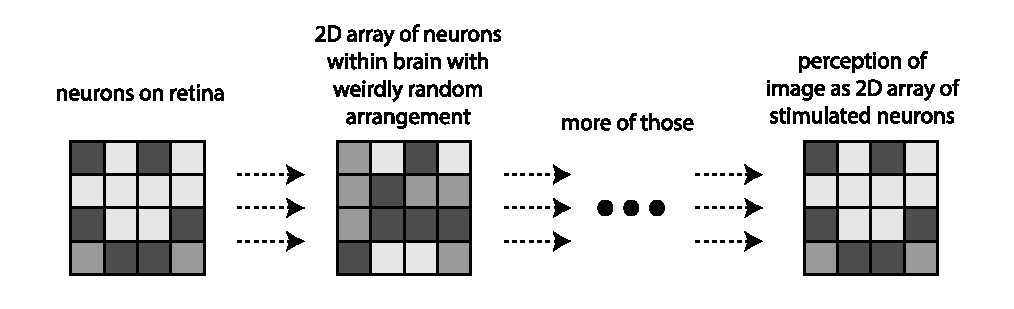
\includegraphics[width=0.95 \linewidth]{retinal}
\caption{ How eyes work, and thus, artificial retinal networks. } \label{fig:retinal}
\end{figure}

This function is {\em biologically plausible}.

We learn by backpropagated stochastic gradient descent, like babies
do. Specifically: The network is presented with an image on its
retina, and then we run the floating point values through the layers,
summing them up and applying the smoothulator function, to produce a
final image within the brain. Like a baby, it compares this image to
what it expected to see, node by node. Where each node does not agree
with the image, the error is computed. The baby propagates the partial
derivative of the change in error with respect to the change in
stimulus to the previous layer proportional to its weighted impact;
fortunately the smoothulator has a simple derivative that is easily
computed at a point from its output values. Error is not propagated
into the real world (i.e., by sending light off of the retina back to
the physical object that created the stimulus; that would be
ridiculous).

\subsection{Training data}

One of the insights of this paper is that although artificial retinal
networks require a lot of data to train, for certain problems the
training data can be easily {\em generated}. For the red i removal
problem, we begin with a corpus of about 4,000 images that were
scraped from Google Image Search. Scraping images is easy; one just
needs to list a bunch of queries for things that babies would want to
view in order to learn what the world looks like. In this experiment I
used terms such as [snakes], [dog on skateboard], [guitar],
[stonehenge] and [superyacht]. Following this, I manually cleaned the
training data. I deleted images that were not photographic (drawings,
etc.; for example, most images of guitars are actually 3D rendered
cartoon guitars, fantasy images of guitars on fire, the Guitar~Hero logo,
and so on) or that were {\em too}, uh, pornographic (most queries for
things that can have sex, like tapirs, contain prominent images of the
things having sex). These are not appropriate for babies.

All images are cropped to a square and resized to 256x256. Then we
generate training instances: An input image and the expected result.
An image that does not contain a red i should just be transformed into
the image itself (indeed, when we peer directly into the brain of a
baby looking at a TV show, we find a region of the brain where the TV
show is clearly visible). It is also easy to generate instances of the
red i removal problem along with their solutions---we simply put a red
i randomly on the source image and keep the destination image
unchanged. In this way, we can easily generate a large amount of
training instances (in actual practice, this procedure had a small bug;
see Section~\ref{sec:evaluation}). One unexpected phenomenon is that
I had to be careful to remove images that already contained a red i,
like many images of casinos, which are often called ``CASINO''.

% notes on corpus:
% - my own picture of library in there

In order to coax networks into recognizing the i, we also place an i
into the 4th color channel in the same position in the {\em expected
output}. This is an invisible color channel which we discard, and
which is always zero in the input. In essence we giving a hint to the
eye's brain that it should not just remove the red i, but it should
also {\em perceive} it. I have not performed enough experiments to
know if this is helpful.

For repeatability's sake, important constants used in this experiment:
There were 2 hidden layers. Gaussan samples were produced with a
standard deviation of 16 pixels. The red i was rendered in Comic Sans,
at a height of 80 pixels. I used a variety of learning rates,
including an expontentially decreasing one (the standard advice of
0.05 is too large for constant learning rates on this kind of task, and
limits the sharpness of resultant images).

\subsection{CUDA, SHUDA, WUDA}

Because we are working with graphical data, we should use the Graphics
Processing Unit of the computer, not its Central Processing Unit (we
are not processing centers). I implemented high-performance OpenCL
kernels for each phase of training: The {\em forward} pass (signals
flowing from the retina to the eye's brain), the {\em backpropagation}
step (when the eye computes the error and partial derivatives) and the
{\em weight update} step (when the eye rewires its neurons so that it
sees the right thing next time). The phases have different parallelism
constraints. Because the connectivity is sparse, we represent both
forward and inverted index maps, which are decoded on the GPU. We take
care to only load a single layer of the retinal network into the GPU's
RAM at once, to enable very large models, but we run many training
instances in parallel for a single round. Some other operations, like
the preparation of training data, are performed on the CPU. These are
also frequently done in parallel, using C++11's new {\tt std::thread}
with some crazy-ass wrappers to allow them to function in mingw32's
64-bit gcc port. On a good day, training uses all 6 CPU cores and all
2800 GPU cores and about 14 GB of RAM and warms the home office like a
1kW space heater.

\section{Results}

After 4 rounds of training, the network produces an excellent-looking
image that could be a {\em Cure} album cover, regardless of the stimulus
cast upon its retina (Figure~\ref{fig:cure}).

\begin{figure}[bth]
\begin{center}
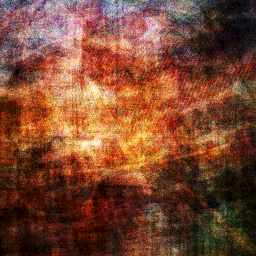
\includegraphics[width=0.65 \linewidth]{cure}
\end{center}
\caption{Result after 4 rounds of training. Looks great, and there is no
red i to be seen, but it loses some points for not resembling the
input image at all.} \label{fig:cure}
\end{figure}

\begin{figure}[htb]
\begin{center}
\includegraphics[width=0.95 \linewidth]{frosted}
\end{center}
\caption{Result after 80 rounds of training, with the input image at the top
and the signal proceeding downward through two hidden layers. The hidden layers
aspire to crazy noise-terror glitch art versions of the stimulus as well.} \label{fig:frosted}
\end{figure}

\begin{figure}[htb]
\begin{center}
\includegraphics[width=0.95 \linewidth]{instagram}
\end{center}
\caption{After about 9,000 rounds. Top row is the input image, the
second row is the output (no longer showing hidden layers because
they all just look like firefly raves); the bottom row shows 4x
magnified detail of the region formerly containing the red i.
Images are somewhat desaturated and blurry, but the red i is removed.
Note how in the right image, the retinal network successfully continued
both the horizontal and vertical bookshelves into the occluded region.
This is not a trick.} \label{fig:instagram}
\end{figure}

\begin{figure}[htb]
\begin{center}
\includegraphics[width=0.95 \linewidth]{eval}
\end{center}
\caption{Evaluation on new images after 30,000 rounds of training. Top row
is the input image, the second row is the output, and third is 4x magnified
defail. The first image (no i) shows the high amount of detail preserved.
In the latter two, the i is successfully removed; the quality of the replacement
is not perfect, but certainly reasonable.} \label{fig:eval}
\end{figure}

\begin{figure}[htb]
\begin{center}
\includegraphics[width=0.95 \linewidth]{jpeg}
\end{center}
\caption{Evaluation of an early model for J peg dequantization. The model
still contains a lot of noise pixels, which sometimes take a long time to
converge, but it is already easy to see how quantization artifacts have been reduced (left).
Actually, there is no reason why such dequantization must only be applied to J pegs;
the right column shows it working on a nice rainbow picture.
} \label{fig:jpeg}
\end{figure}

It's not long before the network learns that it should not produce the
same result for every input, and the output starts to mimic the
input. These images look sort of like the world viewed through frosted
glass (Figure~\ref{fig:frosted}), simulating how a baby first learns
to see the world through the 1cm bulletproof Lexan of its translucent
BabyLearn incubation cylinder.

Soon thereafter, the network begins to converge on something like the
identity function, as this drastically reduces error (even if some
error is incurred by the persistence of the red i). Left overnight
(about 9,000 rounds), we start to see the network both produce images
much like the original (perhaps through a hip ``vintage'' Instagram
filter), as well as removing the red i stimulus (Figure~\ref{fig:instagram}).


\subsection{Evaluation} \label{sec:evaluation}

With a further 30,000 rounds of training, the output images sharpen
and lose their Instagram quality (maybe only a small amount of
``grain''), and the i is still successfully removed. However, since
we've now made many passes over each image in the training set (and
the model has about 100,000 degrees of freedom), it is certainly
possible that we've simply overfit to this set of images (that is,
that the baby's eye's brain is simply memorizing the i-free images and
then recalling the one that looks closest to the stimulus). To evaluate
fairly, we need to apply the model to totally new images that it was
not trained on. These are called ``eval'' images.

Firing this up, I observed that the model successfully reproduced eval
images that did not contain a red i; this is good because it means
that it is not simply memorizing the training set images. I then
started placing red i stimulus on the images with the mouse, and my
heart sank: It wasn't removing the red i at all! Dejected, I tried
loading up the training images and putting a red i on them---it also
did not remove the i, which did not make sense! Even for babies!
Eventually, I discovered that the red i would be removed, as expected,
but only when the i was in a handful of very specific locations. This
was found to be a bug in the random i placing code; can you find it too?

\smallskip
\noindent \verb+        uint8 x_dice = seed & 0x255;+ \\
          \verb+        seed >>= 8;+ \\
          \verb+        uint8 y_dice = seed & 0x255;+
\smallskip

As a result, there are only 16 different possible $x$ coordinates, and same
for $y$. Nonetheless, this is still 256 different i locations that work,
which implies considerable generality is possible. Due to Draconian SIGBOVIK
deadlines, I have not yet been able to test a debugged training procedure.

Once the evaluation code only places an i at expected locations, the artificial
retinal network works well (Figure~\ref{fig:eval})!


\section{Conclusions}

We find that the supposedly impossible red i removal problem is in
fact solvable, at least in some forms, using artificial retinal
networks. There are some limitations of the current model:
\begin{itemize}
\item It has only been tested to remove the letter i when it is rendered
  in bright red, in 30 point Comic Sans.
\item It probably also removes letters like j, but maybe also in some
  other fonts, which is a sword that cuts both ways.
\item Due to a bug, the red i must be at a position whose coordinates are exactly
  $\langle 12 + x_0 + 4x_1 + 16x_2 + 64x_3, 12 + y_0 + 4y_1 + 16y_2 + 63y_3 \rangle$,
for $x_j$ and $y_j$ in $\{0, 1\}$.
\item It automatically and non-optionally applies Instagram-style filters.
\end{itemize}

This technique can probably be applied to other image processing
problems, for example, J peg dequantization. Here, we take an image
and badly quantize it (for example, to 4 bits per color channel), and
the training instance consists of the quantized image as input and the
original image as the expected output; the retinal network learns how
to fill in detail. Figure~\ref{fig:jpeg} shows the early stages (about
4000 rounds) of training such a model.

A related, still unsolved problem is ``red i reduction''; here we do
simply remove the i but replace it with a smaller i. For example, we
could replace a capital I with a lowercase one, or replace a lowercase
30pt Comic Sans i with a lowercase 29pt Comic Sans i. This is an
offshoot of the text ure compression field, which seeks to make the
text ``ure'' smaller wherever it appears.

\medskip
Biologically-inspired computer algorithms hold many wonders for those
that seek to tap into the limitless potential of the 85\% of the human
eye's brain that is currently unused. Perhaps humans even contain
graphics processing units!

\bigskip
For higher-fidelity images and source code, please consult {\tt
http://tom7.org/redi}.

\end{document}
